\documentclass[10pt,a4paper,twoside]{article}
\usepackage[english]{babel}
%laad de pakketten nodig om wiskunde weer te geven :
\usepackage{amsmath,amssymb,amsfonts,textcomp}
%laad de pakketten voor figuren :
\usepackage{graphicx}
\usepackage{float,flafter}
\usepackage{hyperref}
\usepackage{inputenc}
\usepackage{minted}
\usepackage{subcaption}

\setlength\paperwidth{20.999cm}\setlength\paperheight{29.699cm}\setlength\voffset{-1in}\setlength\hoffset{-1in}\setlength\topmargin{1.499cm}\setlength\headheight{12pt}\setlength\headsep{0cm}\setlength\footskip{1.131cm}\setlength\textheight{25cm}\setlength\oddsidemargin{2.499cm}\setlength\textwidth{15.999cm}

\newcommand{\sweepsize}{0.3}

\begin{document}
\begin{center}
\hrule

\vspace{.2cm}
{\bf {\Large Computer Vision - Lab Assigment Report} \\ {\Large Image segmentation}}
\vspace{.1cm}
\end{center}
{\bf Tuan Mate Nguyen}  (tunguyen@student.ethz.ch)
\hrule
\section*{Mean-shift}

\subsection*{Bandwidth}
As expected, increasing bandwidth results in fewer distinguished segmented
object. The reason is that the weights of more distant (in color-space
coordinates) colors contained in the
image pixels are higher relative to closer colors when using smaller bandwidth.
 As a result the mean color value assigned
to the current pixel will be closer to the global mean (mean color of the full image).
Consequently these mean values be also closer to each other with each step until
merging into a set of colors with only few different colors.

On the other hand in case of a smaller bandwidth value basically the only the
close neighborhood would be taken into account. If the color clusters are
well-separated and far apart the found mean will better approximate the cluster
mean.

If, however, the bandwidth is too small, the new color will basically remain
unchanged (other colors having low weights have no effect) resulting in an image
very similar to the original. (Actually the script crashes if there are too many colors.)
5->3 colors
4->2 
3.8->6
1.8-> ~24
1.5->more than 25 -> error

\begin{figure}[h]
    \centering

    \begin{subfigure}{\sweepsize\textwidth}
    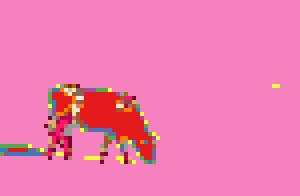
\includegraphics[width=0.9\linewidth]{result_1.8.png} 
    \caption{$bandwidth=1.8$}
    \end{subfigure}
    \begin{subfigure}{\sweepsize\textwidth}
    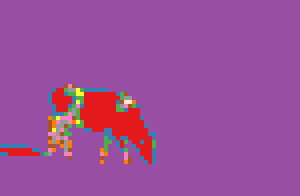
\includegraphics[width=0.9\linewidth]{result_2.5.png} 
    \caption{$bandwidth=2.5$}
    \end{subfigure}
    
    \begin{subfigure}{\sweepsize\textwidth}
    
\includegraphics[width=0.9\linewidth]{result_3.8.png} 
    \caption{$bandwidth=3.8$}
    \end{subfigure}
    \begin{subfigure}{\sweepsize\textwidth}
    
\includegraphics[width=0.9\linewidth]{result_5.png} 
    \caption{$bandwidth=5$}
    \end{subfigure}
    \caption{Segmented images for different bandwidth values}

\end{figure}

\subsection*{Performance}

% Python code
%\begin{minted}[mathescape,
%    linenos,
%    numbersep=5pt,
%    gobble=2,
%    frame=lines,
%    framesep=2mm,
%    firstnumber=26]{csharp}
%\end{minted}

% Image
%\begin{figure}[H]
%    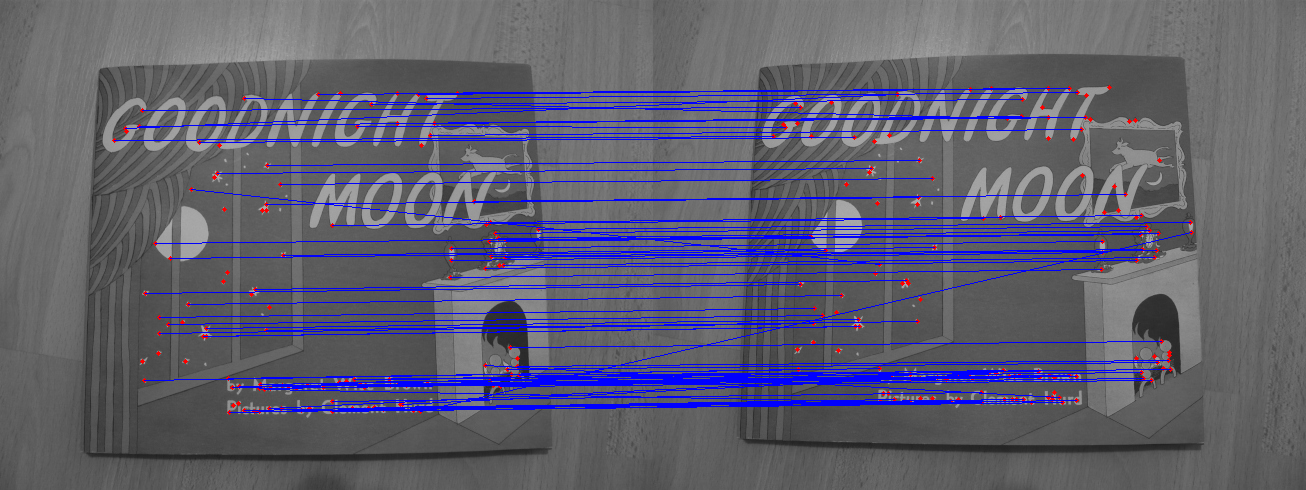
\includegraphics[width=\textwidth]{match_mutual.png}
%    \centering
%    \caption{Matching keypoints for mutual nearest neighbor matching}
%    \label{match_mutual}
%\end{figure}

\end{document}
